\documentclass{article}
\usepackage{amsmath, amsthm, amsfonts}
\usepackage{graphicx}
\usepackage{xcolor, soul}  
\usepackage{mathtools}


\title{CSC301 Lecture 9}
\author{1910456 Mir Shafayat Ahmed}
\color{black}
\begin{document}
    \pagecolor[HTML]{FFFFCC}
    \maketitle
    \section*{Review so far}
    When we were talking about regular expressions, we talked about regular language. We minimized DFA. Which meant we can minimize NFAs as they can be converted to DFA. We made NFAs into Regex and vice versa. So we can also make DFAs from Regex.
    We discussed all of them in a "framework" known as regular language.
    \\
    We were only allowed to use + (or), Concatenation and * (star).
    \section*{A Shortcoming of Regex} 
    A simple requirement of programming languages is making sure that the number of left brackets are equal to the number of right brackets.
    \\
    But with Regex, there is no way to "count" exactly how many we need. When using 0* we have no control over how many 0s are produced.
    \\
    What we want is something like $0^n1^n$ where the number of 0s is exactly the same as 1s.
    \\
    To include strings as simple as 000111 and 0011, we use \textbf{Context Free language} which is expressed with \textbf{Context Free Grammar}.
    \section*{Context Free Languages}
    \subsection*{Trees}
    \begin{figure}[h]
            \centerline{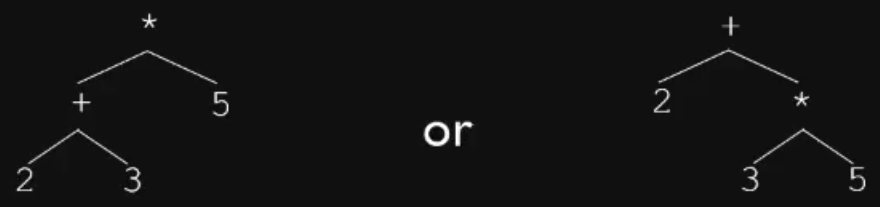
\includegraphics[scale=0.3]{Precedence Tree.png}}
            \caption{Precedence Tree}
            \label{precedence tree}
    \end{figure}
    When we want to calculate 2+3*5, we think from the bottom up approach (recursion trees). Hence, the tree on the right of Figure \ref{precedence tree} is the method we follow (how we do math)
    \\
    So we do 3*5 first and then, 2+15.
    \begin{figure}[h]
        \centerline{
            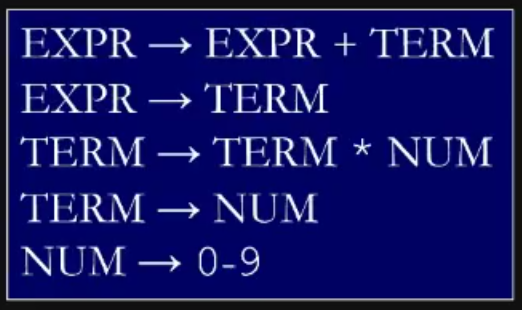
\includegraphics[scale=0.3]
            {RuleForArithmetic.png}
        }
        \caption{Rule Of Basic Arithmetic Operations}
        \label{Arithmetic Rule}
    \end{figure}
    \\
    In Figure \ref{Arithmetic Rule} we can say that an expression (EXPR) can be a summation of an expression and a term. An expression can also be just a term. A term can be the product of a term and a number. A number is anything between [0, 9].
    \\
    Now we see if we can derive the previous Arithmetic operation from this rule:
    \begin{figure}[h]
        \centerline{
            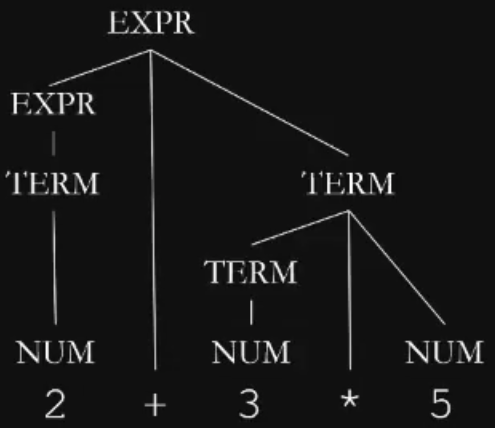
\includegraphics[scale=0.3]{Expression To Tree.png}
        }
        \caption{Tree From Expression}
        \label{ExpToTree}
    \end{figure}
    \\
    In Figure \ref{ExpToTree}, we used the rules in Figure \ref{Arithmetic Rule}.
    \subsection*{Context Free Grammar}
    $$A\to 0A1$$
    $$A\to B$$
    $$B\to \#$$
    The Capital letters on the left are called \emph{variables}. The different rows represent rules (or \emph{productions}) denoted by "$\to$". Anything to the right that are not variables are called terminals. Here, 0, 1 and \# are \emph{terminals}. The variable in the first rule is called the \emph{start variable}.
    
    We can derive 00\#11 from the rules above:
    \begin{equation}
        \begin{split}
            A &\to 0A1\\
            &\to 00A11\\
            &\to 00B11\\
            &\to 00\#11
        \end{split}
    \end{equation}
    \subsection*{Definition of CFG}
    
    A CFG is a quad-tuple, given by $(V, \Sigma, R, S)$ where,\\
    V is a finite set of \emph{variables} or \emph{non-terminals}\\
    $\Sigma$ is a finite set of \emph{terminals}\\
    R is a set of \emph{productions} or \emph{substitution rules} in the form $A\to \alpha$\\
    S is the \emph{start variable}
    \begin{figure}[h]
        \centerline{
            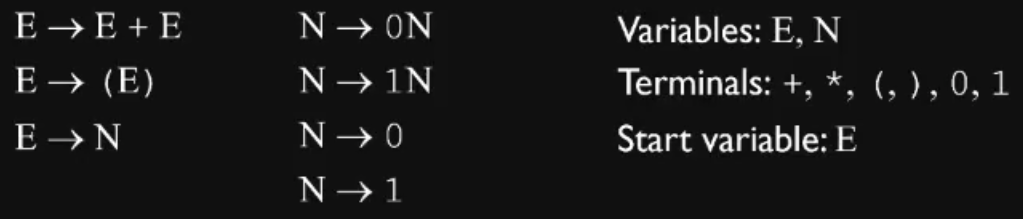
\includegraphics[scale=0.3]{Example CFG 1.png}
        }
        \caption{Identifying the CFG from the definition}
        \label{CFG 1}
    \end{figure}
    
    In shorthand, we can write:
    $$E\to E+E\;|\;(E)\;|\;N$$
    $$N\to 0N\;|\;1N\;|\;0\;|\;1$$

    \begin{figure}[h]
        \centerline{
            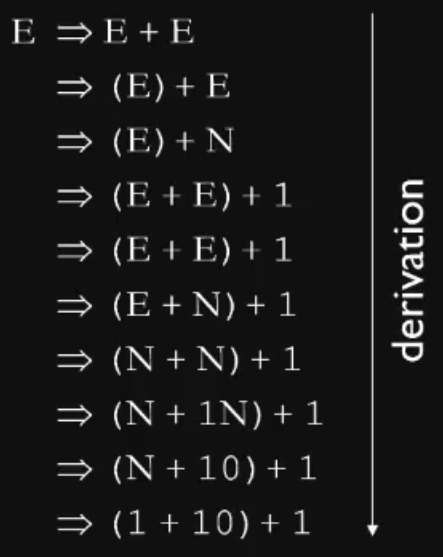
\includegraphics[scale=0.25]{Derivation.png}
        }
        \caption{A Derivation based on CFG in Figure \ref{CFG 1}}
    \end{figure}
    We say that $E\xRightarrow{\text{*}} (1+10)+1$. The '*' above the $\Rightarrow$ represents 'after many productions'.
    \\
    \textbf{\emph{The Language of a CFG is the set of all strings at the end of a derivation}}
    $$L(G)=\{w:w\in \Sigma^*\;and\;S\xRightarrow{*}w\}$$
    
    \subsection*{Parse Trees}
    Given a CFG, $S\to SS\;|\;(S)\;|\;\varepsilon$. We can create a string "(()())".
    \begin{equation}
        \begin{aligned}
            S&\Rightarrow (S)\\
            &\Rightarrow (SS)\\
            &\Rightarrow ((S)S)\\
            &\Rightarrow ((S)(S))\\
            &\Rightarrow (()(S))\\
            &\Rightarrow (()())
        \end{aligned}
        \label{Derivation 2}
    \end{equation}
    \\
    We can create a parse tree which gives us a more compact representation of a derivation.
    \begin{figure}[h]
        \centerline{
            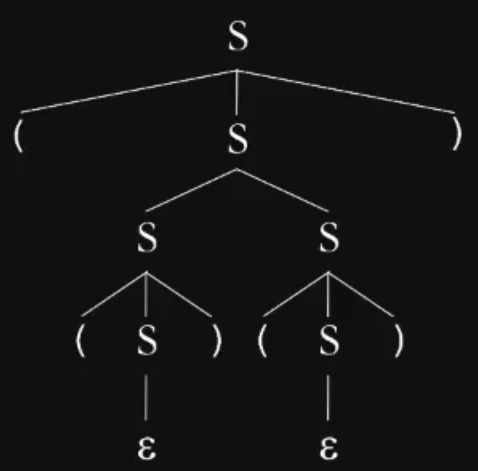
\includegraphics[scale=0.25]{Parse Tree.png}
        }
        \caption{The Parse tree for the derivation \ref{Derivation 2}}.
        \label{ParseTree1}
    \end{figure}
    \\
    No matter what steps we do first in a specific derivation of a \emph{specific} string, the parse tree looks the same for all.\\
    When Drawing a parse tree, we can draw it bottom-up or top-to-bottom.

    \subsection*{Examples}
    Some examples were discussed.A detailed discussion will be on the next lecture summary.




\end{document}